\documentclass[12pt,a4paper]{article}

% ─── Page Layout ───────────────────────────────────────────────────────────────
\usepackage[a4paper, margin=0.8in, headheight=14pt]{geometry}

% ─── Fonts (XeLaTeX) ───────────────────────────────────────────────────────────
\usepackage{fontspec}
\usepackage{unicode-math}
\setmainfont{TeX Gyre Pagella}
\setmonofont[Scale=0.88]{TeX Gyre Cursor}
\setmathfont{Latin Modern Math}

% ─── Packages ──────────────────────────────────────────────────────────────────
\usepackage{xcolor}
\usepackage{colortbl}
\usepackage{titlesec}
\usepackage{enumitem}
\usepackage{tabularx}
\usepackage{booktabs}
\usepackage{array}
\usepackage{amsmath}
\usepackage{tikz}
\usetikzlibrary{shapes.geometric, arrows.meta, positioning, calc, fit, decorations.pathreplacing}
\usepackage{tcolorbox}
\tcbuselibrary{skins, breakable}
\usepackage{hyperref}
\usepackage{fancyhdr}
\usepackage{graphicx}
\usepackage{microtype}
\hyphenpenalty=10000
\exhyphenpenalty=10000
\sloppy
\usepackage{caption}
\usepackage{setspace}
\usepackage{multirow}
\usepackage{tocloft}

% ─── Q&A helper ────────────────────────────────────────────────────────────────
\newcommand{\Q}[1]{\textbf{#1}\par\noindent\ignorespaces}

% ─── Colour Palette ────────────────────────────────────────────────────────────
\definecolor{myred}{RGB}{196,30,58}
\definecolor{mydark}{RGB}{30,30,50}
\definecolor{mygreen}{RGB}{14,120,80}
\definecolor{myteal}{RGB}{0,130,140}
\definecolor{myamber}{RGB}{180,100,0}
\definecolor{mypurple}{RGB}{100,30,160}
\definecolor{mygray}{RGB}{246,247,249}
\definecolor{mgframe}{RGB}{180,185,200}
\definecolor{watermark}{RGB}{145,150,170}
\definecolor{hdrred}{RGB}{250,232,235}
\definecolor{hdrgreen}{RGB}{220,244,233}
\definecolor{hdrteal}{RGB}{220,242,244}
\definecolor{hdramber}{RGB}{253,242,215}
\definecolor{hdrpurple}{RGB}{238,228,255}
\definecolor{hdrgray}{RGB}{238,240,245}
\definecolor{rowalt}{RGB}{250,251,253}

% ─── Section Formatting ────────────────────────────────────────────────────────
\titleformat{\section}
  {\large\bfseries\color{myred}}{\thesection.}{0.5em}{}
  [\vspace{1pt}{\color{myred}\rule{\linewidth}{0.8pt}}]
\titleformat{\subsection}
  {\normalsize\bfseries\color{myteal}}{\thesubsection}{0.5em}{}
\titlespacing*{\section}{0pt}{18pt}{7pt}
\titlespacing*{\subsection}{0pt}{11pt}{4pt}

% ─── Paragraph ─────────────────────────────────────────────────────────────────
\setlength{\parindent}{0pt}
\setlength{\parskip}{4pt}

% ─── TOC Styling ───────────────────────────────────────────────────────────────
\renewcommand{\cfttoctitlefont}{\large\bfseries\color{myred}}
\renewcommand{\cftaftertoctitle}{\par\noindent{\color{myred}\rule{\linewidth}{0.8pt}}}
\setlength{\cftbeforetoctitleskip}{0pt}
\setlength{\cftaftertoctitleskip}{6pt}
\renewcommand{\cftsecfont}{\normalsize\bfseries\color{mydark}}
\renewcommand{\cftsecpagefont}{\normalsize\bfseries\color{mydark}}
\renewcommand{\cftsecleader}{\cftdotfill{\cftdotsep}}
\setlength{\cftbeforesecskip}{7pt}
\renewcommand{\cftsubsecfont}{\small\color{mydark}}
\renewcommand{\cftsubsecpagefont}{\small\color{mydark}}
\setlength{\cftbeforesubsecskip}{3pt}
\setlength{\cftsubsecindent}{1.4em}

% ─── Table helpers ─────────────────────────────────────────────────────────────
\renewcommand{\arraystretch}{1.45}
\setlength{\tabcolsep}{6pt}
\arrayrulecolor{mydark}
\newcolumntype{B}[1]{>{\small\bfseries\raggedright\arraybackslash}m{#1}}
\newcolumntype{Y}{>{\small\raggedright\arraybackslash}X}
\renewcommand{\tabularxcolumn}[1]{m{#1}}

% ─── Header / Footer ───────────────────────────────────────────────────────────
\pagestyle{fancy}
\fancyhf{}
\fancyhead[L]{\small\color{myred}\textbf{OE-EC604C}\;\color{mydark}--- Object Oriented Programming}
\fancyhead[R]{\small\color{myteal}\textbf{Module 1 Notes}}
\fancyfoot[C]{\small\color{mydark}\thepage}
\fancyfoot[R]{\small\color{watermark}\textit{\copyright\ Biraj}}
\renewcommand{\headrulewidth}{0.5pt}
\renewcommand{\footrulewidth}{0.3pt}

% ─── Hyperref ──────────────────────────────────────────────────────────────────
\hypersetup{
  colorlinks=true, linkcolor=myteal, urlcolor=myteal,
  pdfauthor={Biraj Sarkar},
  pdftitle={OE-EC604C --- Module 1 Notes}
}

% ─── tcolorbox styles ──────────────────────────────────────────────────────────
\tcbset{
  tikzbox/.style={
    colback=mygray, colframe=mgframe, boxrule=0.6pt, arc=4pt,
    left=8pt, right=8pt, top=6pt, bottom=6pt,
    colbacktitle=mgframe, coltitle=mydark,
    fonttitle=\small\bfseries
  },
  defbox/.style={
    colback=hdrgreen, colframe=mygreen, boxrule=0.8pt, arc=4pt,
    left=9pt, right=9pt, top=6pt, bottom=6pt,
    colbacktitle=mygreen, coltitle=white,
    fonttitle=\small\bfseries
  },
  formulabox/.style={
    colback=hdrteal, colframe=myteal, boxrule=0.8pt, arc=4pt,
    left=9pt, right=9pt, top=7pt, bottom=7pt,
    colbacktitle=myteal, coltitle=white,
    fonttitle=\small\bfseries
  },
  examplebox/.style={
    colback=hdramber, colframe=myamber, boxrule=0.8pt, arc=4pt,
    left=9pt, right=9pt, top=6pt, bottom=6pt,
    colbacktitle=myamber, coltitle=white,
    fonttitle=\small\bfseries
  },
  masonbox/.style={
    colback=hdrpurple, colframe=mypurple, boxrule=0.8pt, arc=4pt,
    left=9pt, right=9pt, top=6pt, bottom=6pt,
    colbacktitle=mypurple, coltitle=white,
    fonttitle=\small\bfseries
  },
  exambox/.style={
    colback=hdrpurple, colframe=mypurple, boxrule=1pt, arc=5pt,
    left=10pt, right=10pt, top=8pt, bottom=8pt,
    colbacktitle=mypurple, coltitle=white,
    fonttitle=\bfseries,
    breakable, title after break={\textbf{Frequently Asked / Viva Questions (contd.)}}}
}

% XeLaTeX pdfcol fix: reset text color after every tcolorbox
\tcbset{after={\color{black}}}

% ─── TikZ styles ───────────────────────────────────────────────────────────────
\tikzset{
  block/.style={rectangle, draw=myteal, fill=hdrteal,
    text width=2.4cm, align=center, minimum height=0.95cm,
    font=\small, rounded corners=3pt, line width=0.7pt},
  redblock/.style={rectangle, draw=myred, fill=hdrred,
    text width=2.4cm, align=center, minimum height=0.95cm,
    font=\small, rounded corners=3pt, line width=0.7pt},
  netnode/.style={rectangle, draw=myteal, fill=hdrteal,
    text width=1.5cm, align=center, minimum height=0.8cm,
    font=\small, rounded corners=3pt, line width=0.7pt},
  sumjunc/.style={circle, draw=myamber, fill=hdramber,
    minimum size=0.62cm, font=\small, line width=0.8pt},
  snode/.style={circle, draw=mypurple, fill=hdrpurple,
    minimum size=0.55cm, font=\footnotesize, line width=0.7pt},
  arrow/.style={-Stealth, thick, color=mydark},
  redarrow/.style={-Stealth, thick, color=myred},
  line/.style={thick, color=mydark}
}

% ═══════════════════════════════════════════════════════════════════════════════
\begin{document}
% ═══════════════════════════════════════════════════════════════════════════════

\begin{center}
  {\LARGE\bfseries\color{myred} OE-EC604C --- Object Oriented Programming}\\[5pt]
  {\normalsize\color{mydark} Semester VI \quad$\bullet$\quad 3L:0T:0P \quad$\bullet$\quad 3 Credits}\\[3pt]
  {\normalsize\color{myteal}\textbf{Module 1 Exam Notes: Programming Paradigm \& OOP Concepts}}\\[3pt]
  {\small\color{mydark} CGEC \;$|$\; B.Tech ECE (2023--27) \;$|$\; \textit{Biraj Sarkar}}
\end{center}
\vspace{2pt}
\noindent{\color{myred}\rule{\linewidth}{1.5pt}}
\vspace{2pt}

\hypersetup{linkcolor=mydark}
\tableofcontents
\hypersetup{linkcolor=myteal}
\newpage

% ===============================================================================
\section{Evolution of Programming Paradigm}
% ===============================================================================

A programming paradigm defines the style, approach, and philosophy of designing and writing software code. As programs grew in size and complexity, paradigms evolved to improve code readability, reuse, and maintainability.

\subsection{Paradigms Evolution Timeline}
\begin{enumerate}[label=\textbf{\arabic*.}, leftmargin=*, itemsep=4pt]
  \item \textbf{Unstructured Programming:} The earliest style where the program consists of a single continuous block of statements (often containing global variables) using jump statements like \texttt{goto} for flow control. It becomes difficult to maintain as code grows ("spaghetti code").
  \item \textbf{Procedural / Structured Programming:} Programs are organized into subroutines, modules, or functions. Flow control is structured using blocks like loops (\texttt{for}, \texttt{while}) and conditional statements (\texttt{if}, \texttt{switch}). Focus is on the \textbf{process or algorithm} rather than data.
  \item \textbf{Object-Oriented Programming (OOP):} A paradigm where programs are organized around \textbf{objects} (representing real-world entities) containing data (attributes) and methods (behaviors). Focus is on \textbf{data security and encapsulation} rather than procedures.
\end{enumerate}

\subsection{Structured vs. Object-Oriented Development}
\begin{itemize}[leftmargin=*, itemsep=3pt]
  \item \textbf{Structured/Procedure-Oriented Programming (POP):} Views a program as a sequence of procedural steps or function calls. Global data is vulnerable because it can be accessed and modified freely by any function.
  \item \textbf{Object-Oriented Programming (OOP):} Views a program as a collection of self-contained, interacting objects. Data is tied closely to the functions that operate on it, preventing accidental outside modification.
\end{itemize}

\begin{tcolorbox}[tikzbox, title={Procedural Paradigm (POP) vs. Object-Oriented Paradigm (OOP)}]
\centering
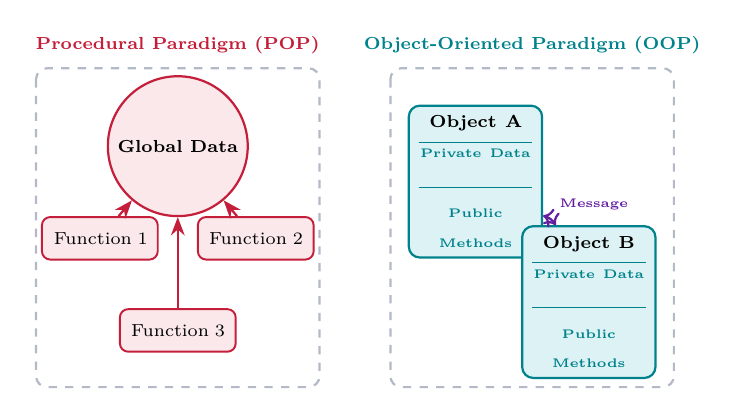
\begin{tikzpicture}[node distance=1.2cm, thick, scale=0.9, every node/.style={scale=0.9}]
  % Procedure-Oriented Model (Left side)
  \draw[dashed, color=mgframe, line width=0.8pt, rounded corners=4pt] (-4, 2.4) rectangle (0, -2.1);
  \node[above=2pt, font=\scriptsize\bfseries\color{myred}] at (-2, 2.4) {Procedural Paradigm (POP)};
  \node[circle, draw=myred, fill=hdrred, minimum size=1.1cm, font=\scriptsize\bfseries] (glob) at (-2, 1.3) {Global Data};
  \node[redblock, text width=1.4cm, minimum height=0.6cm, font=\scriptsize] (f1) at (-3.1, 0.0) {Function 1};
  \node[redblock, text width=1.4cm, minimum height=0.6cm, font=\scriptsize] (f2) at (-0.9, 0.0) {Function 2};
  \node[redblock, text width=1.4cm, minimum height=0.6cm, font=\scriptsize] (f3) at (-2, -1.3) {Function 3};
  \draw[redarrow] (f1) -- (glob);
  \draw[redarrow] (f2) -- (glob);
  \draw[redarrow] (f3) -- (glob);

  % Object-Oriented Model (Right side)
  \draw[dashed, color=mgframe, line width=0.8pt, rounded corners=4pt] (1, 2.4) rectangle (5, -2.1);
  \node[above=2pt, font=\scriptsize\bfseries\color{myteal}] at (3, 2.4) {Object-Oriented Paradigm (OOP)};
  
  \node[draw=myteal, fill=hdrteal, rounded corners=4pt, text width=1.6cm, align=center, inner sep=4pt] (obj1) at (2.2, 0.8) {
    \scriptsize\bfseries Object A\\
    \color{myteal}\rule{\linewidth}{0.4pt}
    \tiny Private Data\\
    \color{myteal}\rule{\linewidth}{0.4pt}
    \tiny Public Methods
  };

  \node[draw=myteal, fill=hdrteal, rounded corners=4pt, text width=1.6cm, align=center, inner sep=4pt] (obj2) at (3.8, -0.9) {
    \scriptsize\bfseries Object B\\
    \color{myteal}\rule{\linewidth}{0.4pt}
    \tiny Private Data\\
    \color{myteal}\rule{\linewidth}{0.4pt}
    \tiny Public Methods
  };
  
  \draw[arrow, color=mypurple, <->, bend left=20] (obj1) to node[midway, above right, font=\tiny\bfseries\color{mypurple}] {Message} (obj2);
\end{tikzpicture}
\end{tcolorbox}

% ===============================================================================
\section{Core Object-Oriented Programming Concepts}
% ===============================================================================

OOP seeks to model software systems in terms of real-world entities. Below are the foundational concepts of OOP:

\subsection{Objects and Classes}
\begin{tcolorbox}[defbox]
\textbf{Class:} A user-defined data type that acts as a blueprint, template, or prototype for creating objects. It defines the properties (data members) and actions (member functions) common to all objects of that class.
\par\vspace{3pt}
\textbf{Object:} A basic run-time entity of an object-oriented system that represents a real-world entity. It is an instance of a class, possessing its own state (data values) and behavior.
\end{tcolorbox}

\subsection{Data Encapsulation and Data Abstraction}
\begin{tcolorbox}[defbox]
\textbf{Data Encapsulation:} The mechanism of binding together code (member functions) and the data it manipulates (data members) into a single unit (class). It implements data hiding, keeping data safe from outside interference.
\par\vspace{3pt}
\textbf{Data Abstraction:} The act of representing essential features of a system without including the background details or implementation explanations. Users interact only with the interface, hiding complex execution.
\end{tcolorbox}

\subsection{Inheritance}
\begin{tcolorbox}[defbox]
\textbf{Inheritance:} The process by which objects of one class acquire the properties and behaviors of another class. It supports hierarchical classification and promotes \textbf{code reusability} by allowing new classes (derived classes) to extend existing ones (base classes).
\par\vspace{3pt}
\textbf{Base Class (Parent Class):} The class whose properties are inherited.
\par\vspace{3pt}
\textbf{Derived Class (Child Class):} The class that inherits from the base class.
\end{tcolorbox}

\subsection{Polymorphism}
\begin{tcolorbox}[defbox]
\textbf{Polymorphism:} The ability of an interface to take multiple forms (from Greek, meaning "many forms"). It allows a single function name, operator symbol, or interface to behave differently depending on the context.
\end{tcolorbox}
There are two main classifications:
\begin{itemize}[leftmargin=*, itemsep=2pt]
  \item \textbf{Compile-Time (Static) Polymorphism:} Resolved at compile time (e.g., function overloading, operator overloading).
  \item \textbf{Run-Time (Dynamic) Polymorphism:} Resolved at runtime during execution (e.g., virtual functions, method overriding).
\end{itemize}

\subsection{Dynamic Binding and Message Passing}
\begin{tcolorbox}[defbox]
\textbf{Dynamic Binding:} The mechanism where the code associated with a given function call is not resolved until runtime. It is associated with inheritance and run-time polymorphism.
\par\vspace{3pt}
\textbf{Message Passing:} The communication process between objects. Objects interact by sending requests to execute methods of other objects, passing arguments and receiving results.
\end{tcolorbox}

% ===============================================================================
% MANDATORY QUICK REVISION PAGE
% ===============================================================================
\newpage
\begin{center}
  {\large\bfseries\color{myred} Quick Revision --- Module I}\\[3pt]
  {\small\color{mydark} Paradigm \& OOP Concepts $|$ OE-EC604C}
\end{center}
\noindent{\color{myred}\rule{\linewidth}{1.2pt}}
\vspace{4pt}

\begin{tcolorbox}[formulabox, title={\textbf{Key Concepts at a Glance}}]
\renewcommand{\arraystretch}{1.3}
\begin{tabularx}{\linewidth}{B{3.2cm} X}
Class Structure         & \texttt{class ClassName \{ private: // data public: // methods \};} \\[4pt]
The 4 Pillars of OOP    & \textbf{Encapsulation} (data hiding), \textbf{Abstraction} (interface separation), \textbf{Inheritance} (code reuse), \textbf{Polymorphism} (many forms). \\[4pt]
Access Modifiers        & \textbf{private}: Accessible only within class (default). \newline \textbf{public}: Accessible from anywhere. \newline \textbf{protected}: Accessible within class and child classes.
\end{tabularx}
\end{tcolorbox}

\begin{tcolorbox}[defbox, title={\textbf{One-Line Definitions}}]
\begin{itemize}[leftmargin=*, itemsep=2.5pt, topsep=0pt]
  \item \textbf{Paradigm:} A structured method or style of programming defining program organization.
  \item \textbf{Class:} A user-defined logical blueprint defining data and member functions.
  \item \textbf{Object:} A physical instance of a class representing a real-world entity.
  \item \textbf{Encapsulation:} Wrapping data and code together into a single unit (class) to prevent global access.
  \item \textbf{Data Hiding:} Restricting direct access to internal data members using access specifiers.
  \item \textbf{Abstraction:} Hiding background implementation details and exposing only the interface.
  \item \textbf{Inheritance:} The mechanism of deriving new classes from existing classes to achieve code reuse.
  \item \textbf{Polymorphism:} The capability of a function, operator, or object to act differently in different contexts.
  \item \textbf{Dynamic Binding:} Resolving method calls at runtime rather than compile time.
  \item \textbf{Message Passing:} Communication model where objects invoke member functions of other objects.
\end{itemize}
\end{tcolorbox}

\begin{tcolorbox}[exambox, title={\textbf{Frequently Asked / Viva Questions}}]
\begin{enumerate}[topsep=0pt, label=\textbf{Q\arabic*.}, itemsep=5pt]
  \item \Q{State the main limitation of Unstructured Programming.}
    Unstructured programming relies heavily on jump commands (like \texttt{goto}), making the control flow complex and highly difficult to trace, maintain, or debug.
  \item \Q{What is the core difference in how POP and OOP view data?}
    Procedure-Oriented Programming (POP) views data as passive elements manipulated by active procedures. OOP views data as critical assets tied securely to active functions.
  \item \Q{Define the difference between a Class and an Object.}
    A class is a logical template or blueprint (allocates no memory). An object is a physical instance of that template created in memory (allocates memory).
  \item \Q{Why does OOP offer better data security than POP?}
    OOP hides data members inside classes using the \texttt{private} access specifier, preventing outside functions from modifying the variables. POP global data is accessible to all.
  \item \Q{How does Encapsulation differ from Abstraction?}
    Encapsulation is the \textit{wrapping} or \textit{containment} of data (data hiding). Abstraction is the \textit{hiding of complexity} by showing only the external interface.
  \item \Q{What is the primary benefit of Inheritance?}
    Code reusability. It allows developer to extend base class properties without rewriting the code, reducing testing and development time.
  \item \Q{Explain the term "Polymorphism" with a real-world example.}
    A single instruction performs different actions based on target. E.g., the "+" symbol performs addition for numbers, but performs concatenation for strings.
  \item \Q{Define static binding vs. dynamic binding.}
    Static binding (early binding) resolves function calls at compile time. Dynamic binding (late binding) resolves function calls at runtime during execution.
  \item \Q{What is the role of access specifiers in C++?}
    Access specifiers (\texttt{private}, \texttt{public}, \texttt{protected}) control the visibility and accessibility of class members from outside classes.
  \item \Q{What is meant by the term "Message Passing"?}
    It is the process by which an object requests execution of a method belonging to another object, passing data parameters and receiving return values.
  \item \Q{Can you have an object without a class in C++?}
    No. In C++, every object must belong to a predefined class which defines its structure and member specifications.
  \item \Q{What is "Spaghetti Code" and in which paradigm does it commonly occur?}
    Spaghetti code is program code with highly convoluted control flow, usually caused by multiple jump statements (\texttt{goto}). It occurs in unstructured programming.
\end{enumerate}
\end{tcolorbox}

\begin{tcolorbox}[tikzbox, title={Comparison of POP and OOP Paradigms}]
\renewcommand{\arraystretch}{1.45}
\par\noindent
\begin{tabularx}{\linewidth}{|B{3.2cm}|Y|Y|}
\hline
\textbf{Parameter} & \textbf{\color{myteal}Procedure-Oriented (POP)} & \textbf{\color{mygreen}Object-Oriented (OOP)} \\
\hline
\textbf{Approach} & Top-down design methodology. & Bottom-up design methodology. \\
\hline
\textbf{Focus} & Focuses on the algorithm/process. & Focuses on the data assets. \\
\hline
\textbf{Data Access} & Functions share global data (unsafe). & Objects hide data using private scope (secure). \\
\hline
\textbf{Reusability} & Limited to function calls. & Achieved via class inheritance. \\
\hline
\textbf{Examples} & C, Pascal, Fortran. & C++, Java, Python, C\#. \\
\hline
\end{tabularx}
\end{tcolorbox}

\end{document}
